
\documentclass[12pt]{article}
\usepackage{graphicx}
\usepackage{amsmath}
\usepackage{caption}
\usepackage{enumitem}
\usepackage{listings}
\usepackage{subcaption}
\usepackage[font={small,it}]{caption}

\graphicspath{ {images/} }
\title {High Performance scientific computing \\
Assignment 1- Comparision of matrix }
\author {Anshuman kumar \\
Roll no.  120010036}

\begin{document}
\maketitle
\section{Introduction}
This code is written for assignment 2 of course High Performance Scientific
Computing. It shows the performance of openMp, mpi and single thread matrix
multiplication.It consist of three exeutable
\begin{itemize}
    \item mpi\_main: uses mpi
    \item main:  single thread
    \item oMpMain: uses openMp
\end{itemize}

\subsection{Running Instruction}
For generating the report see README.md
The results are generated for report folder

\section{Computer Spec}
\begin{itemize}
    \item Name: ASUS E402M
    \item Processor: Intel BYT-M 2Core 2840 up to 2.58Ghz
    \item Ram memory: 2gb
    \item OS: Arch Linux
    \item Cache: 1mb
\end{itemize}


\section{Result}
It can be concluded the the Mpi is the fastest with the speed of around 1.7 for
a dual core processor. For OpenMp it was around 1.6. See the plot below that gives
the idea about speed up for all the processes.

As I tested it only one time the speed up differ for various cases.
The first plot show the n vs time taken plot. The lower n are invisible because of
very large n.
The second plot is log log version same plot.


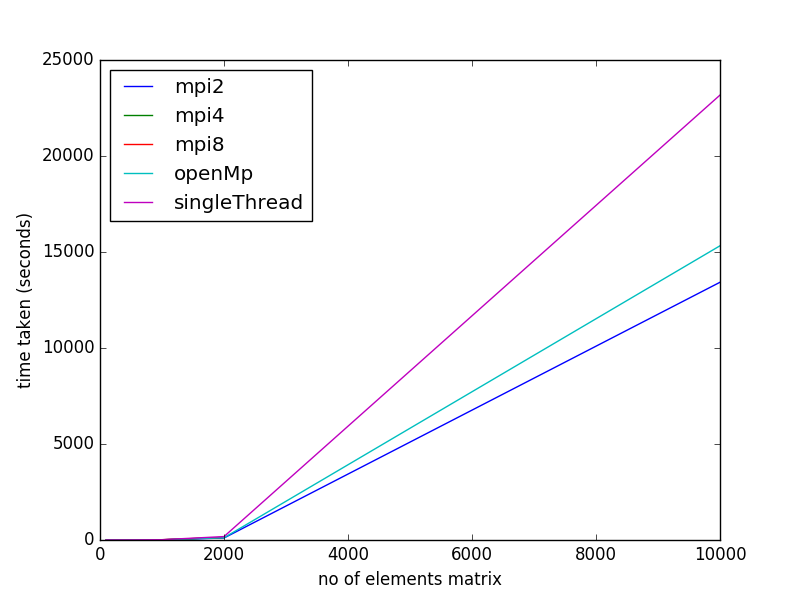
\includegraphics[width=12cm]{normal}

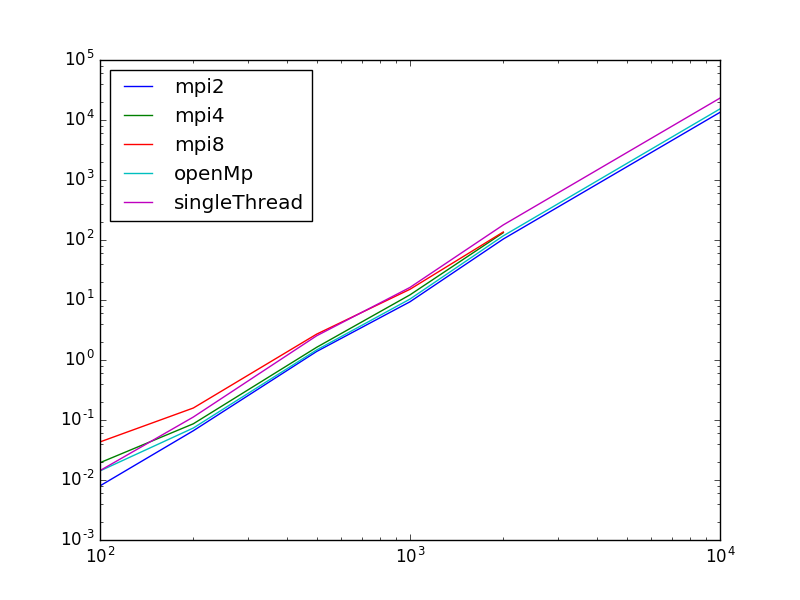
\includegraphics[width=12cm]{log}

\end{document}
